\documentclass[12pt]{article}
\usepackage{pgfplots}
\pgfplotsset{compat=1.17}
\usepgfplotslibrary{fillbetween}
\usepackage{amsmath}
\usepackage{float}
\usepackage[a4paper,left=1in,right=1in,top=1in,bottom=1in]{geometry}
\usepackage{setspace}
\usepackage{mathptmx}
% \usepackage{showframe}

\begin{document}

\makeatletter
\def\@maketitle{%
%   \newpage
%   \null
%   \vskip 1em%
  \begin{center}%
  \let \footnote \thanks
    {\LARGE \@title \par}%
    % \vskip 1em%
    {\large
      \@author \quad \@date}%
    \vskip 1em%
    %{\large \@date}%
  \end{center}%
  \par
  }
\makeatother

\begin{doublespace}

    \title{Economics 101 Reflection Essay}
    \author{Sean Balbale}
    \date{April 30, 2025}
    


\maketitle




When you crack an egg for breakfast, you might not think about the invisible forces that determine its price. Yet our market system relies on two simple ideas: supply and demand. Let me explain how these interact and why a disease outbreak can transform your omelet into a costly luxury.

\textbf{a. The basics of supply and demand.} Imagine a crowded restaurant: if the chef charges too much for pancakes, fewer customers buy them. Conversely, if pancakes are too cheap, the chef runs out of ingredients. \emph{Demand} describes how many eggs consumers want at each price—lower prices boost purchases, creating a downward‐sloping demand curve. \emph{Supply} shows how many eggs farmers produce at each price—higher prices make egg‐laying more profitable, giving an upward‐sloping supply curve. The point where these curves cross is the equilibrium: the quantity and price that clear the market.

\textbf{b. Analysis of the egg shortage.} In early 2022, a severe bird flu outbreak forced farmers to cull millions of hens. This event is a \emph{supply‐side shock}. Overnight, the supply curve shifted left—from $S$ to $S'$—because at any price, fewer eggs were available. With consumer demand unchanged, the market could not immediately clear the old equilibrium quantity $Q_0$, resulting in a shortage. The shortage pushed prices higher until a new equilibrium $E_1$ emerged, with a reduced quantity $Q_1$ and increased price $P_1$.  
The process unfolded in four steps: (1) culling millions of laying hens cuts weekly egg output, (2) wholesalers scramble to fill orders from limited stock, (3) retailers bid up prices at auctions to secure scarce eggs, and (4) these higher wholesale costs propagate through distributors to grocery stores and restaurants. The magnitude of the price jump depends on elasticities: if supply is very inelastic (farmers cannot quickly increase production), and demand is inelastic (consumers view eggs as essential), prices spike dramatically.

\begin{figure}[H]
\centering
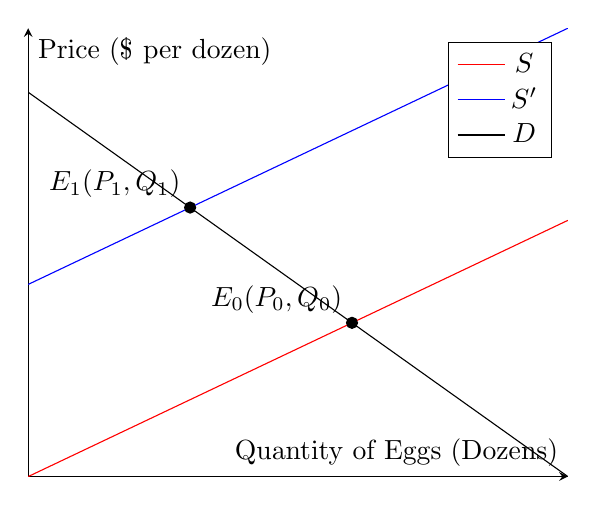
\begin{tikzpicture}
  \begin{axis}[
    axis lines=middle,
    xlabel={Quantity of Eggs (Dozens)},
    ylabel={Price (\$ per dozen)},
    xtick=\empty, ytick=\empty,
    legend pos= north east
  ]
  \addplot[name path=S,domain=0:8, color=red] {0.5*x+2};
  \addlegendentry{$S$}
  \addplot[name path=S2,domain=0:8, color=blue] {0.5*x+5};
  \addlegendentry{$S'$}
  \addplot[name path=D,domain=0:8] {-0.75*x+8};
  \addlegendentry{$D$}
  \addplot[only marks] coordinates {(4.8,4.4)} node [above left] {$E_0(P_0,Q_0)$};
  \addplot[only marks] coordinates {(2.4,6.2)} node [above left] {$E_1(P_1,Q_1)$};
  \end{axis}
\end{tikzpicture}
\caption{Supply and demand shifts in the egg market.}
\end{figure}

\textbf{c. Impact on the breakfast café market.} For a café that runs on eggs, higher egg prices raise input costs. This cost increase acts like a leftward shift of the café’s supply curve for egg‐based dishes, from $S_{\text{café}}$ to $S'_{\text{café}}$. At the previous menu price $p_0$, the restaurant cannot profitably serve the same number of dishes, so it raises prices to $p_1$. The extent of this price increase depends on:
\begin{itemize}
  \item \textbf{Cost share of eggs:} Dishes heavy in eggs (e.g., omelets) face larger cost pressure.
  \item \textbf{Demand elasticity:} If customers are sensitive to price, cafés may absorb part of the cost to keep patrons.
  \item \textbf{Substitute availability:} More alternatives (e.g., egg‐free items) limit how much prices can rise.
\end{itemize}

\begin{figure}[H]
\centering
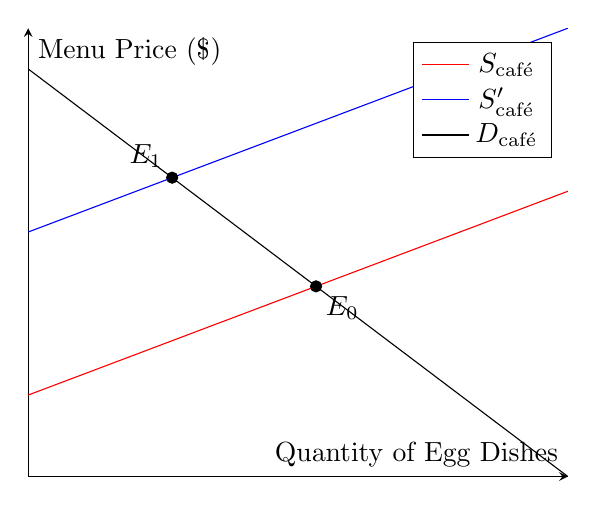
\begin{tikzpicture}
  \begin{axis}[
    axis lines=middle,
    xlabel={Quantity of Egg Dishes},
    ylabel={Menu Price (\$)},
    xtick=\empty, ytick=\empty,
    legend pos= north east
  ]
  \addplot[name path=Sc,domain=0:10, color=red] {0.25*x+4};
  \addlegendentry{$S_{\text{café}}$}
  \addplot[name path=Sc2,domain=0:10, color=blue] {0.25*x+6};
  \addlegendentry{$S'_{\text{café}}$}
  \addplot[name path=Dc,domain=0:10] {-0.5*x+8};
  \addlegendentry{$D_{\text{café}}$}
  \addplot[only marks] coordinates {(5.3333,5.3333)} node [below right] {$E_0$};
  \addplot[only marks] coordinates {(2.6667,6.6667)} node [above left] {$E_1$};
  \end{axis}
\end{tikzpicture}
\caption{Supply shift in the breakfast café market.}
\end{figure}


\textbf{d. Positive spillovers and vaccination subsidies.} Vaccinating 300 million hens against bird flu not only protects vaccinated flocks (private benefit) but also reduces disease spread across farms, stabilizing supply and prices (social benefit). This is a \emph{positive externality}: farmers do not capture the full value of reduced outbreak risk. Left to market forces, vaccination will be under‐provided. A government subsidy or cost‐sharing program would align private costs with social benefits, ensuring vaccination reaches a level that maximizes overall welfare.

By tracing these steps—from the bird flu supply shock to café menu surcharges and the case for subsidized vaccination—you can see why your morning omelet costs more and how simple market principles explain the ripple effect behind the shell.

\end{doublespace}
\end{document}
